% main.tex

\documentclass[british, 8pt, unknownkeysallowed]{beamer}
% \documentclass[british, 8pt, handout]{beamer} % handout

\usepackage{ragged2e}

% ENCODING AND LANGUAGES : 

%\usepackage{german}
%\usepackage[german,english]{babel}
\usepackage[english]{babel}
% \usepackage[german]
% \usepackage[utf8latin1]{inputenc}
\usepackage[utf8]{inputenc} 


% LOGIC 

\usepackage{forarray}
\usepackage{calc}



% MATH STUFF 
\usepackage{amsmath, amsthm} 
% % % % incompatible to beamer ? 
\usepackage{pxfonts}
\usepackage{pifont}
\usepackage{mathrsfs}
\usepackage{commath}

\usepackage{amsmath} % assumes amsmath package installed
\usepackage{amssymb}  % assumes amsmath package installed
%\usepackage{bm}
\usepackage{mathtools}
% % % 
\theoremstyle{definition}
% \newtheorem{definition}[theorem]{Definition}
\newtheorem{characterization}[theorem]{Characterization}

%% THIS CAN DESTROY A LOT -- DO NOT ACTIVATE THAT ! 
%% \usepackage[charter]{mathdesign}

%% \usepackage[binary,amssymb]{SIunits}%
\usepackage[11pt]{moresize}

% TABLE STUFF 

\usepackage{booktabs}
\usepackage{multirow}
\usepackage{xcolor,colortbl}

\definecolor{Gray}{gray}{0.8}

% GRAPHIX

\usepackage{graphicx}
\usepackage{xcolor}
\usepackage{subfigure}
\usepackage{tikz}
\usepackage{svg}


%
% do not use for beamer since it overwrites the beamer stuff ... , see innertemplate instead ... 
%% \usepackage[figurename=]{caption}

% LAYOUT

\usepackage[overlay,absolute]{textpos}
\usepackage{microtype}


% ALGORITHMS 

\usepackage{listings}


\usepackage{hyperref}

\hypersetup{
    hypertexnames=true,
    unicode     = {false},
    colorlinks  = {false},
    pdftitle    = {},
    pdfsubject  = {},
    pdfauthor   = {},
    pdfkeywords = {},
    pdfborder   = {0 0 0},
    bookmarks   = true,
    breaklinks  = true,
}


% TEMPLATE 

\setbeamersize{text margin left=.33cm,text margin right=.33cm}
% does not have any effect ? 
% \setbeamersize{text margin top=1.5cm, text margin bottom=1.5cm}

% THIS FONT ALSO SCREWS UP THE SPACINGS --> IT NEEDS TO BE PART OF THE TEMPLATE ! 
% IT LOOKS NICER THAN STANDARD FONT ! 
%% 
%% \usepackage{lmodern}
%% 

% tikz needed for beamerthemephbaer
\usepackage{beamer_template_theme_ric_uni_bremen}
\usepackage{tikz}


\beamertemplatenavigationsymbolsempty
\setbeamertemplate{sections/subsections in toc}[circle]
\setbeamercovered{%
  still covered={\opaqueness<1->{20}},
  again covered={\opaqueness<1->{40}}}

\if@twocolumn
  \setlength\leftmargini  {0.7em}
\else
  \setlength\leftmargini  {1.2em}
\fi
\leftmargin  \leftmargini
\setlength\leftmarginii  {1.0em}

% \usepackage{beamer_template_appendixnumber}
\usepackage{appendixnumberbeamer}
% UNSORTED 

\usepackage{textcomp}


\usepackage[backend=biber,sorting=none,style=alphabetic,citestyle=authoryear,maxcitenames=2,maxbibnames=99]{biblatex}
\addbibresource{references.bib}
\AtBeginBibliography{\setcounter{maxnames}{3}}

\newrobustcmd*{\parentexttrack}[1]{%
  \begingroup
  \blx@blxinit
  \blx@setsfcodes
  \blx@bibopenparen#1\blx@bibcloseparen
  \endgroup}

\AtEveryCite{%
  \let\parentext=\parentexttrack%
  \let\bibopenparen=\bibopenbracket%
  \let\bibcloseparen=\bibclosebracket}


% define bib item template with larger graphic
\defbeamertemplate{bibliography item}{mybibitem}
{\textbullet} % \lower5pt\hbox{\scalebox{2}{}}} % \pgfuseimage{beamericonarticle}

% choose to show enlarged article items using that template
% \setbeamertemplate{bibliography item}[mybibitem]
\setbeamertemplate{bibliography item}[text]
 
 
% text_maccros

\newcommand{\inputTheSmallFigure}[1]
{\raisebox{-0.25cm}{\includegraphics[width=0.8cm]{figures/math/quaternions/coords/#1}}}
 
\newcommand{\yepp}{\ding{51}}
\newcommand{\nope}{\text{--}}

% \newcommand{\CadToSim}{\texttt{CAD-2-SIM}}


\newcommand{\isf}[1]{\inputTheSmallFigure{#1}}

% \inputSmallMatrix
\newcommand{\ism}[9]{$\biggl[\begin{smallmatrix}#1&#2&#3\\#4&#5&#6\\#7&#8&#9\end{smallmatrix}\biggr]$}

% % % 
\newcommand{\smallhyperlink}[2]     {{\small\href{#1}{#2}}}
\newcommand{\sepsmallhyperlink}[2]  {\begin{itemize}\item \smallhyperlink{#1} \end{itemize}}
% % % 
% % % 
\newcommand{\smallurl}[1]     {{\tiny\url{#1}}}
\newcommand{\sepsmallurl}[1]  {\begin{itemize}\item \smallurl{#1} \end{itemize}}
% quotation marks - G erman :
\newcommand{\glr}{bla}
\newcommand{\gqq}[1]{\glqq #1\grqq}
\newcommand{\gq}[1] {\glq  #1\grq}
% quotation marks - E nglish : 
\newcommand{\eqq}[1]{\lq\lq #1\rq\rq}
\newcommand{\eq}[1] {\lq  #1\rq}
% quotation marks - F rench : 
\newcommand{\fqq}[1]{\flqq #1\frqq}
\newcommand{\fq}[1] {\flq #1\frq}

% write something like >@somebody< with the commmand >\at somebody<
\newcommand{\at}{$@$}


\newcommand{\req}[1]    {Equation~\ref{#1}}
\newcommand{\rseq}[1]   {Eq.~\ref{#1}}

\newcommand{\rsec}[1]   {Section~\ref{#1}}
\newcommand{\rfig}[1]   {Figure~\ref{#1}}
\newcommand{\rdiag}[1]  {Diagram~\ref{#1}}
\newcommand{\rpar}[1]   {Paragraph~\ref{#1}}
\newcommand{\rtab}[1]   {Table~\ref{#1}}
\newcommand{\rapp}[1]   {Appendix~\ref{#1}}
\newcommand{\rexa}[1]   {Example~\ref{#1}}


% % todo A NICE FEATURE to MARK development directives: 
\newcommand{\temptext}[1]{\noindent\fcolorbox{lightgray}{white}{\color{gray}\begin{minipage}{\textwidth}{#1}\end{minipage}}\color{black}}


\newcommand{\technical}[1]{\texttt{#1}}

% A
\newcommand{\ADRF}{\technical{ADRF}}
\newcommand{\AutodeskInventor}{\technical{Autodesk Inventor}}
% C
\newcommand{\CAD}{\technical{CAD}}
\newcommand{\CadToSim}{\technical{CAD-2-SIM}} 
\newcommand{\cpp}{\technical{C++}}
\newcommand{\Cpp}{\technical{C++}}
% G 
\newcommand{\GUI}{\technical{GUI}}
% L 
\newcommand{\Latex}{\technical{\LaTeX}}
% M 
\newcommand{\Mars}{\technical{Mars}}
\newcommand{\Matlab}{\technical{Matlab}}
% O 
\newcommand{\Openrave}{\technical{Openrave}}
\newcommand{\opensim}{\technical{OpenSim}}
% P
\newcommand{\Python}{\technical{Python}}
\newcommand{\python}{\technical{Python}}


% S 
\newcommand{\Simulink}{\technical{Simulink}}
\newcommand{\Solidworks}{\technical{SolidWorks}}
\newcommand{\SolidWorks}{\technical{SolidWorks}}
\newcommand{\simtk}{\technical{SimTK}}
\newcommand{\simbody}{\technical{SimBody}}
% V 
\newcommand{\Visualbasic}{\technical{VisualBasic}}
% W
\newcommand{\WRL}{\technical{WRL}}
% X
\newcommand{\XML}{\technical{XML}} 



% slide_macros

\newcommand{\separationframe}[1]{\frame[noframenumbering]{\structpartshort{#1}}}



% \newcommand{\specialSeparationframe}[2]{%
% \frame{\begin{center}%
% \includegraphics[width=0.66\linewidth]{#2}%                                                 
% \end{center}% 
% \vspace*{0.1cm}
% {\color{capiogray}\huge #1}}
% }

\newcommand{\specialSeparationframe}[2]{%
\begin{frame}
% \pgfputat{\pgfxy(10.5, 2.5)}{\pgfbox[left,top]{\includegraphics[width=0.66\linewidth]{#2}}}
% \pgfputat{\pgfxy(10.5, 5.5)}{\pgfbox[left,top]{\includegraphics[height=1cm]{figures/cad_2_sim_logo}}}
% \pgfputat{\pgfxy(1.0, 5.5)}{\pgfbox[left,top]{\color{capiogray}\huge #1}}}
% \pgfputat{\pgfxy(1.0, 5.5)}{\pgfbox[left,top]{\color{capiogray}\huge #1}} 
% 
\begin{center}
\begin{columns}[c]
\begin{column}{0.15\linewidth}
 
\end{column}

\begin{column}{0.35\linewidth}
  \scriptsize 
  \tableofcontents[currentsection]
\end{column}

\begin{column}{0.48\linewidth}
\includegraphics[width=0.99\linewidth]{#2}
\end{column}
% 
\end{columns}
\end{center}

{\color{capiogray}\huge #1}
% 

\end{frame}
}


%% {\color{fg!35}bla}

% % % \usepackage{paralist}
% % % 
% % % \setlength{\pltopsep}       {2pt}       % Space between first item and preceding paragraph.
% % % \setlength{\plpartopsep}    {0pt}       % Extra space added to \topsep when environment starts a new paragraph (is called in vmode).
% % % 
% % % \setlength{\plitemsep}      {0pt}       % Space between successive items.
% % % \setlength{\plparsep}       {0pt}       % Space between paragraphs within an item – the \parskip for this environment.
% % % 
% % % \newenvironment{itemizeflat}
% % % {\begin{compactitem}}
% % % {\end{compactitem}}
% % % 
% % % \newenvironment{enumerateflat}
% % % {\begin{compactenum}}
% % % {\end{compactenum}}


\newcommand{\pim}{\pause \item}

\newcommand{\bluemph}[1]{\textcolor{blue}{#1}}


% centering an image (needed for background image) -- three arguments 
% 
%   #1  --  figure width
%   #2  --  figure vertical offset 
%   #3  --  the figure file 
% 
\newcommand{\centergraphics}[3]
{
\parbox[c]{\paperwidth}{\vspace*{#2\paperwidth}\centering\includegraphics[width=#1\linewidth]{#3}}
}


% making an image opaque (nice for background images) -- four arguments 
% 
%   #1  --  opacity value 
%   #2  --  figure width
%   #3  --  figure vertical offset 
%   #4  --  the figure file 
% 
\newcommand{\opaccentergraphics}[4]
{
\tikz\node[opacity=#1]{\centergraphics{#2}{#3}{#4}};
}


% centralize anything easily ... with restricted width 
% 
\newenvironment{slimcenter}[1]
{%
  \begin{columns}\begin{column}{#1}
}{%
  \end{column}\end{columns}
}


% centralize figure easily ... 
% 
\newenvironment{figureH}
{% 
  \begin{figure}[H]\centering
}% 
{% 
  \end{figure}
}

% centralize table easily ... 
% 
\newenvironment{tableH}
{% 
  \begin{table}[H]\centering
}% 
{% 
  \end{table}
}


% tweaking the quote environment 
% 
\renewenvironment{quote}
  {\list{}{\leftmargin=0.3cm\rightmargin=0.3cm}\item[]\color{capiogray}\it}
  {\endlist}

% giving the source for a quotation 
% 
\newcommand{\quotesource}[1]
  {\hspace*{\fill}\textup{\color{black}#1}}


% --------------------------------------------------------------------------------

% 
% TODO : FOR CUSTOM BOXES -- check 'tcolorbox' -- see http://tex.stackexchange.com/questions/27093/what-are-alternatives-to-block
% 

% --------------------------------------------------------------------------------

% an environment to refer too publications 
% 
\newenvironment<>{slideBibBox}
{%
    \begin{actionenv}%
    \def\insertblocktitle{\footnotesize{Publication}}%
    \par%
     \mode<presentation>{%
        % \setbeamercolor{block title}{ fg=white,bg=orange!20!black}
        % \setbeamercolor{block body}{fg=black,bg=olive!50}
        % \setbeamercolor{itemize item}{fg=orange!20!black}
        % \setbeamertemplate{itemize item}[triangle]
     }%
    \usebeamertemplate{block begin}\footnotesize}
{
    \par\usebeamertemplate{block end}
    \end{actionenv}
}

\newcommand{\currentPubState}[1]    {({\texttt{\tiny#1}})}

\newcommand{\bibWHO}[1]     {#1.\ }
\newcommand{\bibWHAT}[1]    {\emph{\eqq{#1}}.\ }
\newcommand{\bibWHERE}[1]   {#1,\ }
\newcommand{\bibWHEN}[1]    {#1.\ }
\newcommand{\bibSTATUS}[1]  {\currentPubState{#1}}

\newcommand{\bibWhoWhatWhereWhenStatus}[5]  
{% 
    \bibWHO{#1}\bibWHAT{#2}\bibWHERE{#3}\bibWHEN{#4}\bibSTATUS{#5}% 
}% 

\newcommand{\bibWhoWhatWhereWhenPublished}[4]  
{% 
    \bibWHO{#1}\bibWHAT{#2}\bibWHERE{#3}\bibWHEN{#4}% 
}% 

% --------------------------------------------------------------------------------


% an environment to refer too publications 
% 
\newenvironment<>{slideWhitePaperBox}
{%
    \begin{actionenv}%
    \def\insertblocktitle{\footnotesize{Whitepaper}}%
    \par%
     \mode<presentation>{%
        % \setbeamercolor{block title}{ fg=white,bg=orange!20!black}
        % \setbeamercolor{block body}{fg=black,bg=olive!50}
        % \setbeamercolor{itemize item}{fg=orange!20!black}
        % \setbeamertemplate{itemize item}[triangle]
     }%
    \usebeamertemplate{block begin}\footnotesize}
{
    \par\usebeamertemplate{block end}
    \end{actionenv}
}

% --------------------------------------------------------------------------------

\newcommand{\whiteWhat}[1]     {\emph{\eq{#1}}.}

% --------------------------------------------------------------------------------


% some general purpose math macros 
% 



%
% some commands for including four figures into one slide ... 
% 


% a maximal figure - see http://tex.stackexchange.com/questions/32886/how-to-fit-a-large-figure-to-page
% 
\newcommand{\ingraphmax}[1] 
{
  {
    \setlength{\fboxsep}{0pt}     %padding thickness
    \setlength{\fboxrule}{1pt}    %padding thickness
    \centering 
    % 
    \newpage\fcolorbox{lightgray}{white}{\includegraphics[width=\textwidth,height=\textheight,keepaspectratio]{#1}}
  }
}

% 'ingraph' -- shorter proxy for 'includegraphics'
% 
\newcommand{\ingraph}[2]{
  \centering\includegraphics[width=#1\linewidth]{#2}
}


\newcommand{\fourFigureGraphics}[1]     {\centering\includegraphics[width=0.8\linewidth]{#1}}

\newcommand{\fourFigureFrame}[5]    
{\begin{frame}{#1}
% 
\vspace*{0.05cm}
\begin{columns}
\centering 
\begin{column}[t]{0.49\linewidth}
\fourFigureGraphics{#2}
\end{column}
\quad 
\begin{column}[t]{0.49\linewidth}
\fourFigureGraphics{#3}
\end{column}
\end{columns}
\vspace*{0.25cm}
\begin{columns}
\centering 
\begin{column}[t]{0.49\linewidth}
\fourFigureGraphics{#4}
\end{column}
\quad 
\begin{column}[t]{0.49\linewidth}
\fourFigureGraphics{#5}
\end{column}
\end{columns}
% 
\end{frame}
}


\newcommand{\fourFigureFramePaused}[5]    
{\begin{frame}{#1}
% 
\vspace*{0.05cm}
\begin{columns}
\centering 
\begin{column}[t]{0.49\linewidth}
% \visible<2->
{\fourFigureGraphics{#2}}
\end{column}
\quad 
\begin{column}[t]{0.49\linewidth}
% \visible<3->
{\fourFigureGraphics{#3}}
\end{column}
\end{columns}
\vspace*{0.25cm}
\begin{columns}
\centering 
\begin{column}[t]{0.49\linewidth}
% \visible<4->
{\fourFigureGraphics{#4}}
\end{column}
\quad 
\begin{column}[t]{0.49\linewidth}
% \visible<5->
{\fourFigureGraphics{#5}}
\end{column}
\end{columns}
% 
\end{frame}
}


\newcommand{\twoFigureFrame}[3]  
{\begin{frame}{#1}
% 
\begin{columns}
\centering 
\begin{column}[t]{0.49\linewidth}
\ingraphmax{#2}
\end{column}
\quad 
\begin{column}[t]{0.49\linewidth}
\ingraphmax{#3}
\end{column}
\end{columns}
% 
\end{frame}
}



\newcommand{\twoFigureFramePaused}[3]  
{\begin{frame}{#1}
% 
\begin{columns}
\centering 
\begin{column}[t]{0.49\linewidth}
% \visible<2->
{\ingraphmax{#2}}
\end{column}
\quad 
\begin{column}[t]{0.49\linewidth}
% \visible<3->
{\ingraphmax{#3}}
\end{column}
\end{columns}
% 
\end{frame}
}


% THIS CAN BE DANGEROUS together with indexing ! 
% 
% active  short verbatim environment between vertical bars a la '|a verb expression|'
% 
\usepackage{fancyvrb}
% 
% this one creates conflicts with makeindex: 
% \DefineShortVerb{\|}
% 
% this one DOES NOT create conflicts with glossaries (at least with texlive 2012): 
\DefineShortVerb{\"}


% -----------------------------------------


\usepackage{relsize}


% -----------------------------------------


% -----------------------------------------


% a flat fraction
% 
\newcommand{\flatfrac}[2]{\ensuremath{#1\,/\,#2}}

% a small fraction
% 
\newcommand{\smallfrac}[2]{\text{\scriptsize$\frac{#1}{{#2}}$}}


\usepackage{fancybox}
\newcommand{\someBox}[1]        {\Ovalbox{#1}}

% -----------------------------------------

\usepackage{lmodern}
% \usefonttheme{serif}


\newcommand{\hdffive}    {\texttt{HDF5}}
\newcommand{\yaml}       {\texttt{Yaml}}



% % some general purpose math macros 
% 

\input{defines/mathematics/variables_and_constants}
\input{defines/mathematics/environments}
% \input{defines/mathematics/macros}


% some document specific math macros 


% -----------------------------------------


% \newcommand{\medfrac}   [2] {\mathsmaller{\frac{#1}{#2}}}


\setbeamercovered{invisible}
% \setbeamercovered{transparent} 
% \newcommand{\stdvec}    [1]             {\vect{\hat{e}}\losmall{#1}} % \hismall{(#1)}}}


\newenvironment<>{tempbox}[1][]{%
  \setbeamercolor{block title example}{fg=white,bg=red!75!black}%
  \begin{block}{}\ttfamily}
{\end{block}}

\newenvironment<>{blockquestion}[1][]{%
  \setbeamercolor{block title}{fg=white,bg=red!50!black}%
  \begin{block}{Question}}
{\end{block}}

\newenvironment<>{blockexample}[1][]{%
  % \setbeamercolor{block title}{fg=white,bg=red!50!black}%
  \begin{example}[#1]}
{\end{example}}


\newenvironment<>{blockcharacterization}[1][]{%
  \setbeamercolor{block title}{fg=white,bg=blue!15!gray}%
  \begin{block}{Characterization (#1)}}
{\end{block}}



\newenvironment<>{blockredefinition}[1][]{%
    \setbeamercolor{block title}{fg=white,bg=red!50!black}%
  \begin{block}{Redefinition (#1)}}
{\end{block}}


\newenvironment<>{blockstructure}[1][]{%
  % \setbeamercolor{block title}{fg=white,bg=red!50!black}%
  \begin{block}{Structure}}
{\end{block}}





% adaptable alternative to 
%   \footfullcite{2002_book_Kuipers_Quaternions}
% reads 
% 

\newcommand\blfootnote[1]{%
  \begingroup
  \renewcommand\thefootnote{}\footnote{#1}%
  \addtocounter{footnote}{-1}%
  \endgroup
}

\newcommand{\printpublication}[1]{\AtNextCite{\defcounter{maxnames}{99}}\fullcite{#1}}

\newcommand{\footcitenice}      [1] {\blfootnote{\tiny \printpublication{#1}}}
\newcommand{\footcitesnice}     [2] {\blfootnote{\textsf{\tiny \printpublication{#1},\printpublication{#2}}}}
\newcommand{\footcitenicenumber}      [1] {\footnote{\tiny \printpublication{#1}}}
\newcommand{\footcitesnicenumber}     [2] {\footnote{\textsf{\tiny \printpublication{#1},\printpublication{#2}}}}
\newcommand{\parencitesmall}      [1] {{\small \parencite{#1}}}
\newcommand{\parencitetiny}      [1] {{\tiny \parencite{#1}}}


\setbeameroption{show notes}
\setbeamertemplate{note page}[plain]


\usepackage{tikz}



% http://tex.stackexchange.com/questions/86188/labelling-with-arrows-in-an-automated-way
% 
% formula, text, node#
% % \newcommand{\mathWithDescription}[3]{%
% % \tikz[baseline]{%
% %     \node[draw=red,rounded corners,anchor=base] (m#3)%
% %     {$\displaystyle#1$};%
% %     \node[above of=m#3] (l#3) {#2};%
% %     \draw[-,red] (l#3) -- (m#3);%
% % }%
% % }


\newcommand{\mathWithDescription}[3]{%
\tikz[baseline]{%
    \node[draw=red,rounded corners,anchor=base] (m#3)%
    {$\displaystyle#1$};%
    \node[below of=m#3] (l#3) {#2};%
    \draw[-,red] (l#3) -- (m#3);%
}%
}


\newcounter{mathLableNode}

\newcommand{\mathLabelBox}[2]{%
   \stepcounter{mathLableNode}%
   \mathWithDescription{#1}{#2}{\themathLableNode}%
}

\newcommand{\boxedRED}[1]{%
\tikz[baseline]{\node[draw=red,rounded corners,anchor=base] (m){\ensuremath{#1}};}
}

% set verbatim to tiny 
% 
\makeatletter
\def\verbatim@font{\ttfamily\tiny}
\makeatother


% defining some math commands 
% 
% \newcommand{\COMMANDNAME}  [NOARGS] {\boldsymbol{REFARGINDEX}}  
% 
\newcommand{\vect}      [1] {\boldsymbol{#1}}
\newcommand{\mat}       [1] {\boldsymbol{#1}}
\newcommand{\tEXP}          {^{\mathsmaller{T}}}
\newcommand{\losmall}   [1] {_{\mathsmaller{#1}}}
\DeclareMathOperator*{\argmin}{arg\,min}

\newcommand{\chapquote}[3]{\begin{quotation} \textit{#1} \end{quotation} \begin{flushright} -- #2, \textit{#3}\end{flushright} }
% some macros ... 
% 
\newcommand{\keypoint}  [1]     {\bluemph{\emph{#1}}}

\newcommand{\KEYsubmechanism}      {\keypoint{Submechs}}
\newcommand{\KEYpersons}           {\keypoint{Persons}} 
\newcommand{\KEYmethods}           {\keypoint{Methods}} 
\newcommand{\KEYimplementation}    {\keypoint{Implementation}}
\newcommand{\KEYlinks}             {\keypoint{Links}} 


% for defining new columntypes 
% 
\usepackage{array}


% cite title and year 
% 
\newcommand{\citeTY}    [1]         {\emph{\citetitle{#1}, \citeyear{#1}}}
\newcommand{\citeATY}   [1]         {\emph{\citeauthor{#1},
\citetitle{#1}, \citeyear{#1}}}

\newcommand{\highlight}[1]{%
  \colorbox{red!50}{$\displaystyle#1$}}

% ------------------------------------------------------------------------------------------------------------------------------------------
% --> all three 
% ------------------------------------------------------------------------------------------------------------------------------------------

\usepackage[printonlyused]{acronym}
\usepackage{multimedia}
\usepackage[normalem]{ulem}
% \usepackage{enumitem}
\usepackage[multiple,flushmargin,hang]{footmisc}

% ------------------------------------------------------------------------------------------------------------------------------------------
% --> all three 
% ------------------------------------------------------------------------------------------------------------------------------------------

\beamertemplatenavigationsymbolsempty
\setbeamertemplate{sections/subsections in toc}[circle]
\setbeamercovered{%
  still covered={\opaqueness<1->{0}},
  again covered={\opaqueness<1->{40}}}
  
\let\oldfootnote\footnote
\renewcommand\footnote[1][]{\oldfootnote[frame,#1]}  
\addtobeamertemplate{footnote}{}{\vspace{2ex}}

\usepackage{xpatch}% or use http://tex.stackexchange.com/a/40705

\def\makenamesetup{%
  \def\bibnamedelima{~}%
  \def\bibnamedelimb{ }%
  \def\bibnamedelimc{ }%
  \def\bibnamedelimd{ }%
  \def\bibnamedelimi{ }%
  \def\bibinitperiod{.}%
  \def\bibinitdelim{~}%
  \def\bibinithyphendelim{.-}}    
\newcommand*{\makename}[3]{\begingroup\makenamesetup\xdef#1{#2, #3}\endgroup}

\newbibmacro*{name:bold}[2]{%
  \makename{\currname}{#1}{#2}%
  \makename{\findname}{\lastname}{\firstname}%
  \makename{\findinit}{\lastname}{\firstinit}%
  \ifboolexpr{ test {\ifdefequal{\currname}{\findname}}
            or test {\ifdefequal{\currname}{\findinit}} }{\bfseries}{}}

\newcommand*{\boldname}[3]{%
  \def\lastname{#1}%
  \def\firstname{#2}%
  \def\firstinit{#3}}
\boldname{}{}{}

\xpretobibmacro{name:last}{\begingroup\usebibmacro{name:bold}{#1}{#2}}{}{}
\xpretobibmacro{name:first-last}{\begingroup\usebibmacro{name:bold}{#1}{#2}}{}{}
\xpretobibmacro{name:last-first}{\begingroup\usebibmacro{name:bold}{#1}{#2}}{}{}
\xpretobibmacro{name:delim}{\begingroup\normalfont}{}{}

\xapptobibmacro{name:last}{\endgroup}{}{}
\xapptobibmacro{name:first-last}{\endgroup}{}{}
\xapptobibmacro{name:last-first}{\endgroup}{}{}
\xapptobibmacro{name:delim}{\endgroup}{}{}

% just for demonstration
%\ExecuteBibliographyOptions{maxnames=99,firstinits}
%\DeclareNameAlias{default}{last-first/first-last}
%
%\boldname{W{\"o}hrle}{Hendrik}{H.}
%\boldname{Woehrle}{Hendrik}{H.}

\begin{document}
\newcommand{\robotName}{RH5V2}

%%%%%%%%%%%%%%%%%%%%%%%%%%%%%%%%%%%%%%%%%
\newcommand{\mvec}[1]{\bm{#1}}
\newcommand{\vc}[1]{\mathbf{\mathbf{#1}}}
%%%%%%%%%%%%%%%%%%%%%%%%%%%%%%%%%%%%%%%%%

\newcommand{\q}{\textbf{q}}
\newcommand{\dq}{\dot{\q}}
\newcommand{\ddq}{\ddot{\q}}

%%%%%%%%%%%%%%%%%%%%%%%%%%%%%%%%%%%%%%%

\newcommand{\Mass}{\mathbf{M}}
\newcommand{\Bias}{\mathbf{b}}
\newcommand{\Gravity}{\mathbf{g}}
\newcommand{\Force}{\mathbf{\lambda}}
\newcommand{\Torque}{\mathbf{\tau}}
\newcommand{\Jac}{\mathbf{J}}

%%%%%%%%%%%%%%%%%%%%%%%%%%%%%%%%%%%%%%%%%
\newcommand{\BIN}{\begin{bmatrix}}
\newcommand{\BOUT}{\end{bmatrix}}

%%%%%%%%%%%%%%%%%%%%%%%%%%%%%%%%%%%%%%%%%
\newcommand{\sref}[1]{Sec~\ref{#1}}
\newcommand{\eref}[1]{(\ref{#1})}
\newcommand{\fref}[1]{Fig.~\ref{#1}}
\newcommand{\tref}[1]{Table~\ref{#1}}

%%%%%%%%%%%%%%%%%%%%%%%%%%%%%%%%%%%%%%%%
\newcommand{\state}{\mathbf{x}}
\newcommand{\ctrl}{\mathbf{u}}
\newcommand{\dynsys}{\mathbf{f}}


%%%%%%%%%%%%%%%%%%%%%%%%%%%%%%%%%%%%%%%
\newcommand{\qTr}{\underline{\q}}
\newcommand{\dqTr}{\underline{\dq}}
\newcommand{\ddqTr}{\underline{\ddq}}
\newcommand{\TorqueTr}{\underline{\Torque}}

%%%%%%%%%%%%%%%%%%%%%%%%%%%%%%%%%%%%%%
\newcommand{\costl}{l}
\newcommand{\dts}{\Delta t_s}
\newcommand{\st}{\text{subject to}}

%\boldname{W{\"o}hrle}{Hendrik}{H.}
%\boldname{Woehrle}{Hendrik}{H.}



% ------------------------------------------------------------------------------------------------------------------------------------------
% --> all three 
% ------------------------------------------------------------------------------------------------------------------------------------------



\title   {Robust Direct Trajectory Optimization \\ Using Approximate Invariant Funnels}
\subtitle {Journal Club, Team 3}
\author   [Federico Girlanda]{BSc Federico Girlanda}
\date     [2022-11]{November, 16th 2022}
\institute[DFKI Bremen]{DFKI Robotics Innovation Center Bremen}


%%%%%%%%%%%%%%%%%%%%%%%%%%%%%%%%%%%%%%%%%%%%%%%%%%%%%%%%%%%%%%%%%%%%%%%%%%%% 

\begin{frame}
 \maketitle
\end{frame}

% \subsection*{Table of Content}
\begin{frame}{Table of Content}
\tableofcontents
\end{frame}

%%%%%%%%%%%%%%%%%%%%%%%%%%%%%%%%%%%%%%%%%%%%%%%%%%%%%%%%%%%%%%%%%%%%%%%%%%%%

\section{Introduction}
\separationframe{Introduction}

\begin{frame}{An algorithm that reason about robustness}
\centering
\begin{block}{Reference}
\begin{itemize}
\item Z. Manchester and S. Kuindersma, ''DIRTREL: Robust Trajectory Optimization with Ellipsoidal Disturbances and LQR Feedback''
\end{itemize}
\end{block}
\vspace{0.5 cm}
\begin{minipage}{.45\linewidth}
\centering
\begin{figure}
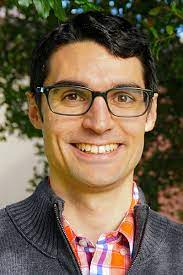
\includegraphics[width=0.4\linewidth, height=0.6\linewidth]{figures/ZMphoto.jpeg}
\caption{Figure 1: Zachary Manchester}
\end{figure}
\end{minipage}
\begin{minipage}{.45\linewidth}
\centering
\begin{figure}
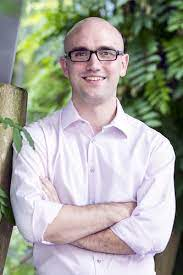
\includegraphics[width=0.4\linewidth, height=0.6\linewidth]{figures/SKphoto.jpeg}
\caption{Figure 2: Scott Kuindersma}
\end{figure}
\end{minipage}
\end{frame}

\begin{frame}{An algorithm that reason about robustness}
\begin{block}{Contribute}
\begin{itemize}
\item In the case of ellipsoidal disturbance sets, fast evaluations of robust cost and constraint functions.   
\item Algorithm that improves tracking performance over non-robust formulations while incurring only a modest increase in computational cost.
\item Evaluation of the algorithm in several simulated robot control tasks.
\end{itemize}
\end{block}
\end{frame}

\section{Background}
\separationframe{Background}

\begin{frame}{Trajectory optimization via DIRTRAN}
\begin{block}{Characteristics}
\begin{itemize}
\item NLP that can be solved using SQP packages such as SNOPT.   
\item Straight forward inclusion of state constraints and avoid numerical pitfalls such as the “tail
wagging the dog” effect.
\item Usually the problem size is large
\end{itemize}
\end{block}
\begin{figure}
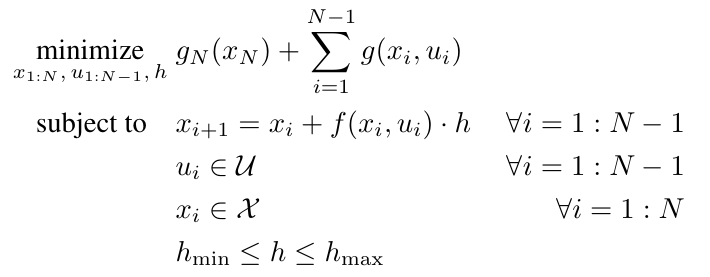
\includegraphics[width=0.6\linewidth, height=0.25\linewidth]{figures/DIRTRANprob.png}
\caption{Figure 3: DIRTRAN optimization problem}
\end{figure}
\end{frame}

\section{Direct Transcription With Ellipsoidal Disturbances}
\separationframe{Direct Transcription With Ellipsoidal Disturbances}

\begin{frame}{State and input deviations}
Assume well defined $ w_i \in W $ disturbances that enter into the dynamics \\
Hence, we can write the disturbed dynamics as \\
\[x_{i+1} = f_h(x_i,u_i,w_i)\]
Given a disturbance sequence $w_{1:N-1}$ we can calulate the state and input deviations from the nominal values.
\vspace{0.5 cm}
\begin{block}{Deviations formulation}
\[\delta x_{i+1} = f_h(x_i + \delta x_i, u_i + \delta u_i, w_i) - x_{i+1}\]
\[\delta u_i = -K_i \delta x_i\]
\end{block}
\end{frame}

\begin{frame}{Robust Cost Function}
\begin{block}{Characteristics}
\begin{itemize}
\item Penalize deviations of the closed-loop system from the nominal trajectory in the presence of disturbances, $w_i$.
\item Quadratic cost of the form $\delta x^T_i Q^l \delta x_i + \delta u^T_i R^l \delta u_i$, where $Q^l \geq 0$ and $R^l \geq 0$ are positive semidefinite cost matrices.
\item Need of a well-defined disturbance sequence, $w_{1:N-1}$.
\end{itemize}
\end{block}
\vspace{0.5 cm}
Robust cost averaged over the entire disturbance set and summed along the trajectory: \\
\[l_W(x_{1:N}, u_{1:N-1}) \approx \frac{1}{Vol(W)}\int_{W} (\delta x^T_N Q^l \delta x_N + \sum_{i=1}^{N-1} (\delta x^T_i Q^l \delta x_i + \delta u^T_i R^l \delta u_i) )\,dW\] \\
but this integral cannot be easily computed.
\end{frame}

\begin{frame}{Robust Cost Function}
\begin{block}{Assumptions}
\begin{itemize}
\item Parametrization of the ellipsoidal set $W$ by a symmetric positive-definite matrix D, such that\\
      \[w^T D^{-1} w \leq 1\]
\item Parametrization of the ellipsoidal bounds on the state deviations $\delta x_i$ by a symmetric positive-definite matrix $E_i$, such that\\
      \[\delta x_i^T E^{-1}_i \delta x_i \leq 1\]
\item Linearization of the disturbed dynamics around the nominal trajectory: \\
      \[\delta x_{i+1} \approx A_i \delta x_{i} + B_i \delta u_i + G_i w\]
\end{itemize}
\end{block}
\vspace{0.5 cm}
Thanks to the previous assumptions we can write the robust cost as: \\
\[l_W(x_{1:N}, u_{1:N-1}) = Tr(Q_N^l E_N) + \sum_{i=1}^{N-1} Tr((Q^l + K^T_i R^l K_i)E_i)\]
\end{frame}

\begin{frame}{The DIRTREL Algorithm}
In addition to augmenting the DIRTRAN optimization problem with $l_W (x_{1:N}, u_{1:N-1})$, we must also ensure that the closed-loop system obeys state and input constraints.
\vspace{0.5 cm}
\begin{block}{Robust state constraints}
$x_i^W = x_i \pm col(E_i^{1/2})$
\end{block}
\begin{block}{Robust input constraints}
$u_i^W = u_i \pm col((K_i E_i K_i^T)^{1/2})$
\end{block}
\end{frame}

\begin{frame}{The DIRTREL Algorithm}
\begin{figure}
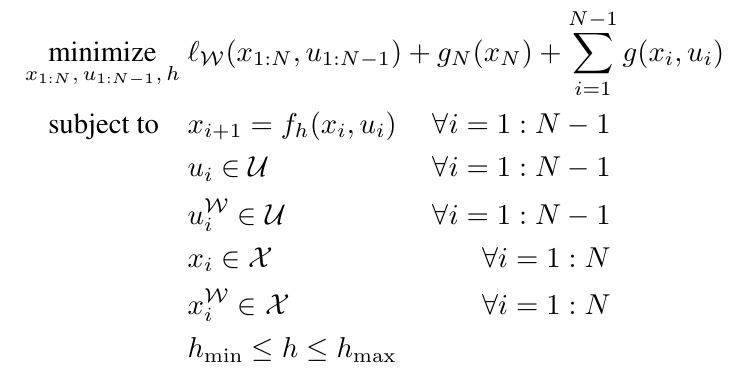
\includegraphics[width=0.8\linewidth, height=0.4\linewidth]{figures/DIRTRELprob.png}
\caption{Figure 4: DIRTREL optimization problem}
\end{figure}
\end{frame}

\section{Examples}
\separationframe{Examples}

\begin{frame}{Pendulum with Uncertain Mass}
\centering
\begin{minipage}{.45\linewidth}
\centering
\begin{figure}
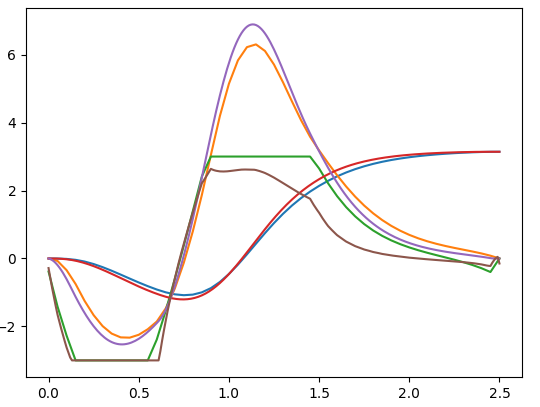
\includegraphics[width=0.8\linewidth, height=0.6\linewidth]{figures/dirtranSimDist.png}
\caption{Figure 5: Direct Transcription nominal and simulated trajectory with disturbed dynamics}
\end{figure}
\end{minipage}
\hspace{0.5 cm}
\begin{minipage}{.45\linewidth}
\centering
\begin{figure}
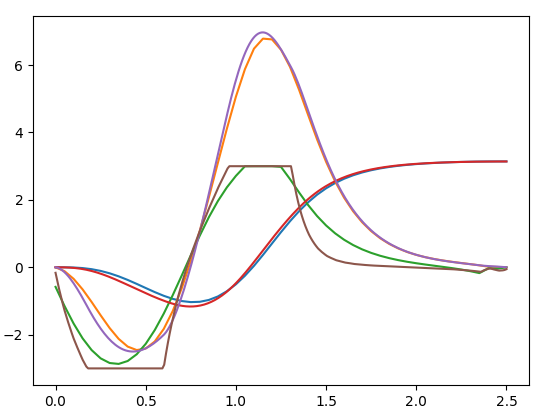
\includegraphics[width=0.83\linewidth, height=0.63\linewidth]{figures/dirtrelSimDist.png}
\caption{Figure 6: DIRTREL nominal and simulated trajectory with disturbed dynamics}
\end{figure}
\end{minipage}
\end{frame}

\begin{frame}{Pendulum with Uncertain Mass}
\centering
\begin{minipage}{.45\linewidth}
\centering
\begin{figure}
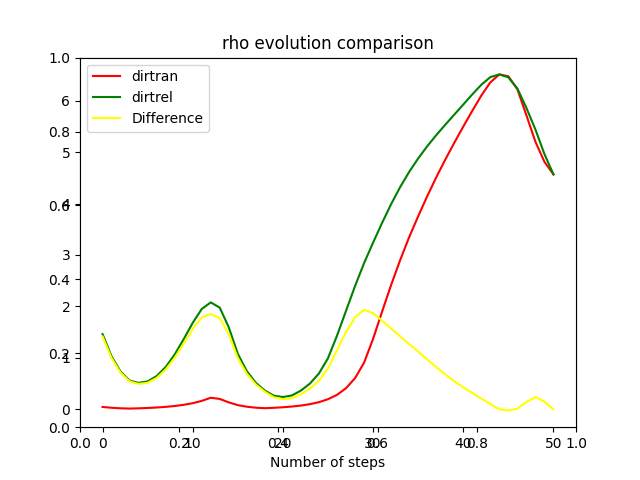
\includegraphics[width=0.85\linewidth, height=0.65\linewidth]{figures/rhoComparison.png}
\caption{Figure 7: Comparison between the RoA dimension rho}
\end{figure}
\end{minipage}
\hspace{0.5 cm}
\begin{minipage}{.45\linewidth}
\centering
\begin{figure}
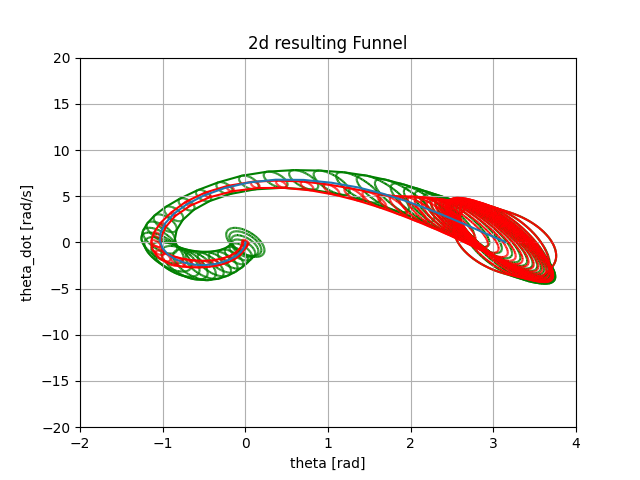
\includegraphics[width=0.85\linewidth, height=0.65\linewidth]{figures/funnelComparison.png}
\caption{Figure 8: Comparison between the RoA representation via funnels}
\end{figure}
\end{minipage}
\end{frame}

\begin{frame}{Cart Pole with Unmodeled Friction}
\centering
\begin{minipage}{.45\linewidth}
\centering
\begin{figure}
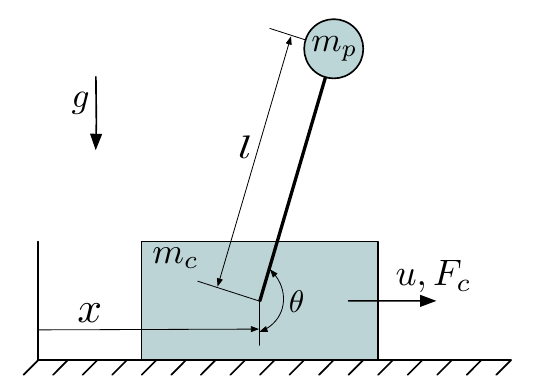
\includegraphics[width=0.8\linewidth, height=0.7\linewidth]{figures/cartpoleSys.png}
\caption{Figure 9: Schematic of the cart pole system}
\end{figure}
\end{minipage}
\hspace{0.5 cm}
\begin{minipage}{.45\linewidth}
\centering
\begin{figure}
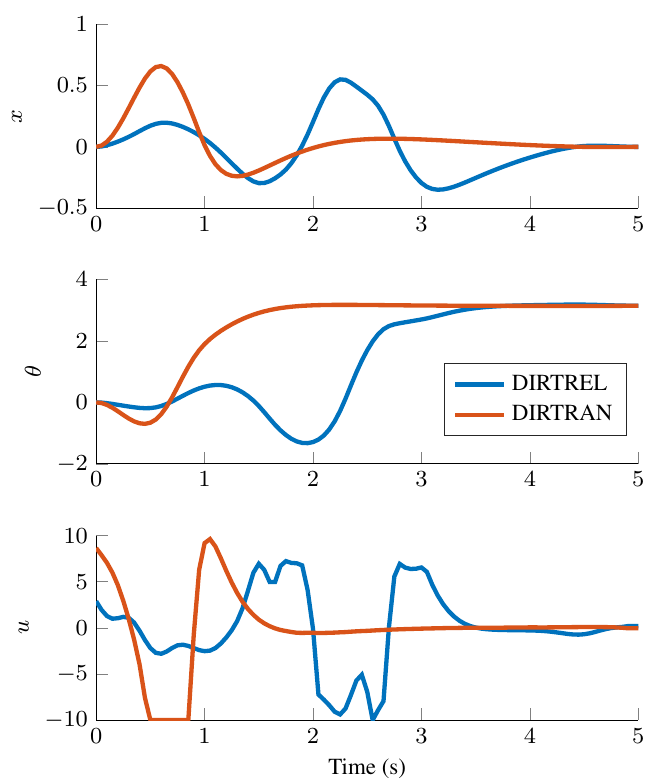
\includegraphics[width=0.7\linewidth, height=0.85\linewidth]{figures/cartpoleTraj.png}
\caption{Figure 10: Resulting nominal trajectories from DIRTRAN and DIRTREL}
\end{figure}
\end{minipage}
\end{frame}

\begin{frame}{Quadrotor with Wind Gusts}
\begin{figure}
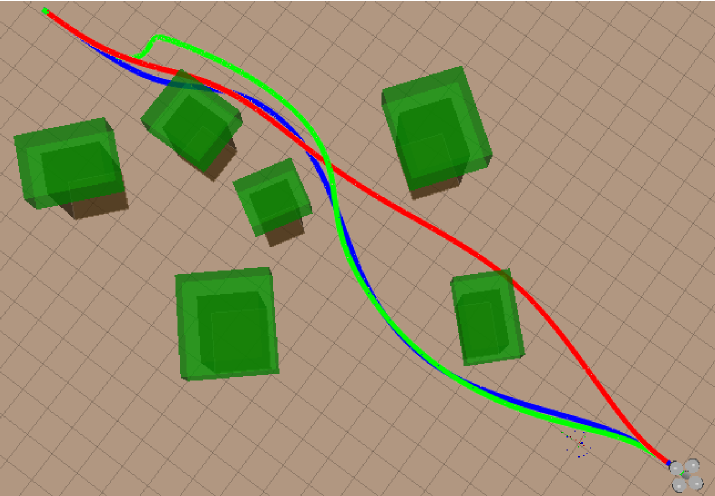
\includegraphics[width=0.7\linewidth, height=0.5\linewidth]{figures/quadrotorTraj.png}
\caption{Figure 11: Resulting nominal trajectories from DIRTRAN and DIRTREL}
\end{figure}
\end{frame}

\begin{frame}{Robot Arm with Fluid-Filled Container}
\begin{figure}
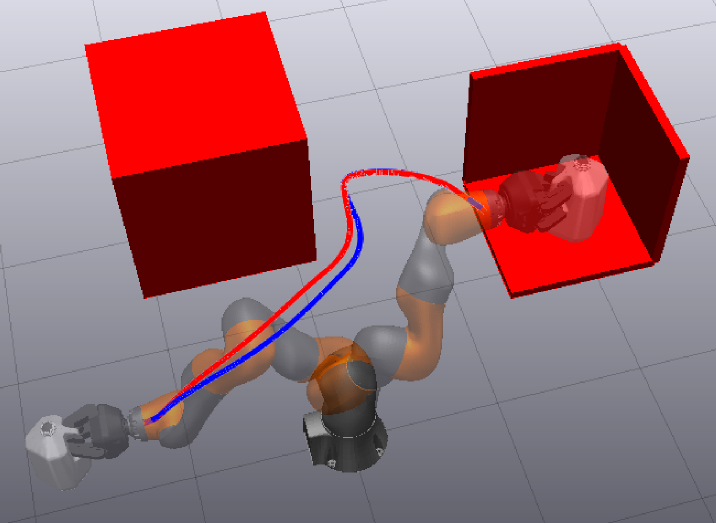
\includegraphics[width=0.7\linewidth, height=0.5\linewidth]{figures/armTraj.png}
\caption{Figure 12: Resulting nominal trajectories from DIRTRAN and DIRTREL}
\end{figure}
\end{frame}

%%%%%%%%%%%%%%%%%%%%%%%%%%%%%%%%%%%%%%%%%%%%%%%%%%%%%%%%%%%%%%%%%%%%%%%%%%%%%%%%%%%

\appendix

\separationframe{Thanks for your attention}

\separationframe{Appendix}

\begin{frame}{Invariant Funnels}
\end{frame}

\begin{frame}{Connections to Sum-of-Squares Methods}
\end{frame}

\end{document}
